\documentclass[12pt]{article}
\usepackage{import}
\usepackage{geometry}
\geometry{letterpaper, total={146.6mm,246.2mm}, left=25.4mm, top=25.4mm, right=25.4mm, bottom=25.4mm } 		%Total is for writing body space. Left/Right, etc are the margins 

\usepackage{preambleWL}

\author{Winfield Lai}
\title{Glass Classification}
\date{\today}

\usepackage{fancyhdr} 		\pagestyle{fancy} 			\fancyhf{}
\lhead{\leftmark } 			\chead{  } 					\rhead{\rightmark}
\lfoot{ Winfield Lai } 		\cfoot{ }
\rfoot{Page \thepage}

\usepackage{setspace} % 1.5 spacing
\linespread{1.25}
\usepackage{cite}
\usepackage{caption}
%\captionsetup[table]{
%  labelsep=newline,
%  justification=justified,
%  singlelinecheck=false,
%  textfont=it,
%}

\begin{document}
\maketitle

\section{Abstract}
A dataset containing the 6 different types of class and 9 measures of chemical properties was analyzed classification prediction. Visualizing the data with a pairs plot and boxplot indicated that several attributes were centered around similar values. $ k $ Nearest Neighbours (KNN) and Classification trees were trained  (stratified sampling) and tested; Adjusted Rand Index (ARI) values were primarily used for comparisons. KNN was tested on the full 9 attributes and 4 attributes of the dataset. In both cases, $ k=1 $ produced the best ARI (0.35 and 0.98 respectively). Classification trees had an ARI of 0.31, indicating that the best method for prediction was using the KNN algorithm with $ k=1 $ and only 4 out of the 9 attributes in the dataset. 

\section{Introduction}
\subsection{Data Set}
Glass classification is useful for crime scene investigations. Glass shards can be used as evidence as long as it is correctly and reliably identified. The following dataset~\cite{dataset} has 10 attributes, one of which is the true glass type: Refractive index(Ri), Sodium (Na), Magnesium (Mg), Aluminum (Al), Silicon (Si), Potassium (K), Calcium (Ca), Barium (Ba), Iron (Fe) and type of glass (Type). There are seven Types - Building Window Float Processed (1), Building Window Non-Float Processed (2), Vehicle Window Float Processed (3), Vehicle Window Non-Float Processed (4), Containers (5), Tableware (6) and Headlamps (7). The elemental attributes (Na, Mg,... etc) are weight percentages of the corresponding oxide. There are no observations of Vehicle Window Non-Float Processed in this dataset and no missing fields. 

Glass identification is quite useful in crimes such as hit and runs, burglaries and vandalism ~\cite{glassEvidence}. Here, glass shards from broken windows or headlamps can be carried by the suspect and any other participants in the scene. This can link suspects and participants to the scene of the crime. 

\subsection{Visualizations}
In Figure \ref{f:dataBasic_Vis}, most attributes are centered around similar values for all types of glass. In the boxplots (right), the boxes overlap for many of the attributes, hence the majority of the data for those attributes are centered around the similar values. When we look at each individual observation in the parallel coordinate graph (left), we see that for most attributes the lines are spread out and it's hard to pinpoint any clusters. There is an exception for Ba and Mg. The Ba boxplot indicates the majority of Type 7 glass is centered around a different value than the other types. The Mg boxplot indicates that Type 1-3, and type 5-6 center around different values as well. These observations are also consistent when looking at the parallel coordinate graph. Ba and Mg may be good choices if we need an attribute to separate out one Glass Type from another. The other attributes may make differentiating different Types harder since their values are all centered similarly. 

\begin{figure}[H]
	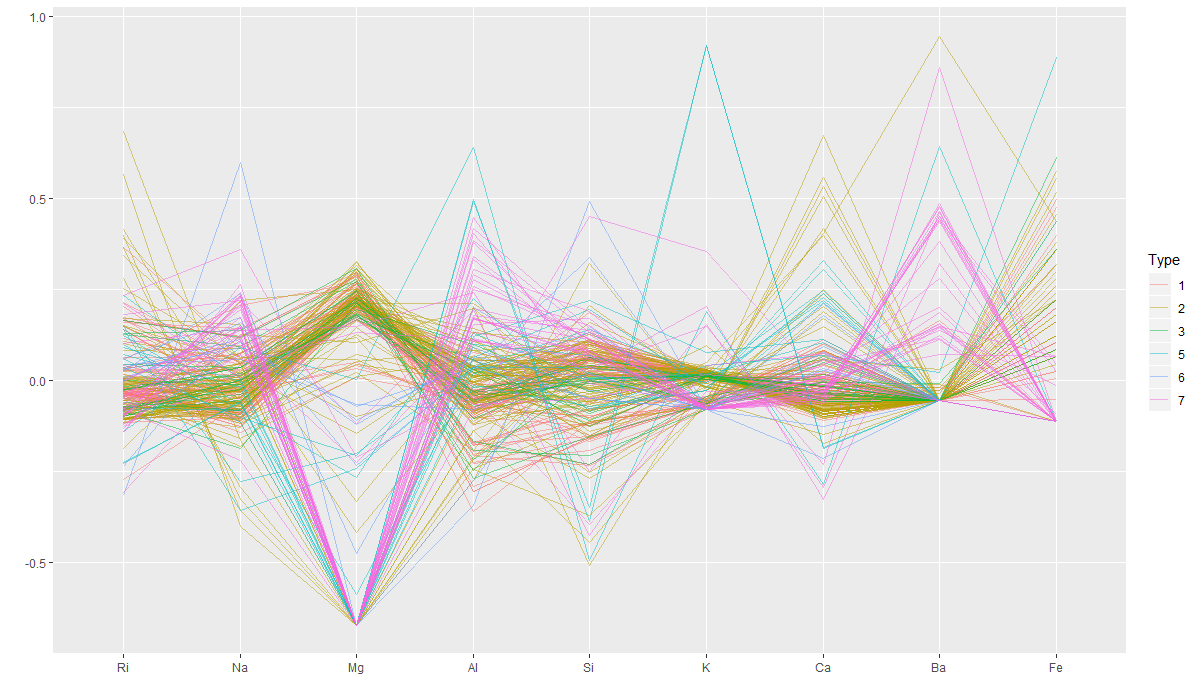
\includegraphics[width=0.49\textwidth, height=2.9in]{parccord.png}
	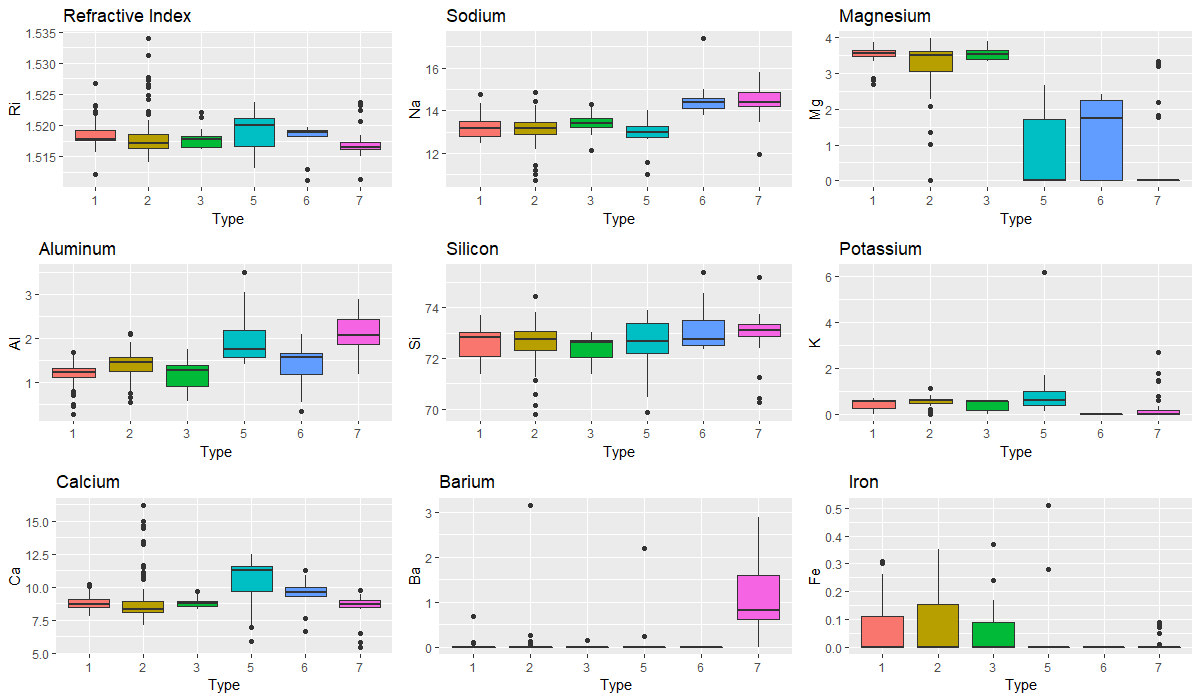
\includegraphics[width=0.49\textwidth, height=2.9in]{boxplot.png}
	\caption{ \\
	\textbf{Left:} Parallel coordinate graph of data. For most attributes, the observations are scattered broadly. There seems to be an exception to this for attributes Ba and Mg.	\\
	\textbf{Right:} Boxplots of all attributes. Many of the boxplots have all glass types centered around similar values. Notable exceptions are Ba and Mg. 
	}
	\label{f:dataBasic_Vis}
\end{figure}

\section{Methods}
\subsection{$ k $ Nearest Neighbours}
The $ k $ Nearest Neighbours (KNN) method predicts the classification of unlabeled points based on the $ k $ closest neighbours~\cite{Lecture}. The Euclidean distance measure is used and unlabeled points are classified according to the majority label of the $ k $ nearest neighbours. 

Typically, a dataset is split into a training set and a test set. 
The KNN method is run for different values of $ k $ on the training set and used to predict the classifications on the test set. 
The $ k $ that has the best classification rate or Adjusted Rand Index (ARI) is then used. 

The KNN method was used on the dataset with all 9 attributes and then only on 4 attributes. Particular attributes were removed because, as seen in Figure \ref{f:dataBasic_Vis}, some attributes are centered around similar values for all glass types. This is not useful for correct predictive classifications in KNN. The more attributes that are centered similarly, the more data points that are closer in Euclidean distance despite being different types. Hence, we removed attributes to further separate out the Types and hopefully improve the predictions. 

Ri, Na, Si, K, and Ca attributes were removed because they had roughly the most overlapping box plots in figure \ref{f:dataBasic_Vis}. The overlap was judged by eye and therefore subject to opinion. However the model's ARI was increasing so inaccuracies in judging the best boxplot to remove were considered insignificant. Additionally, no further attributes were removed because the ARI was close to 1 and we had already removed 5 of the total 9 attributes. Removing more attributes would leave too few attributes. 

Stratified sampling (75\% for all Types except Type 6 which used 50\%) was used to construct the test and corresponding training sets. The KNN method was then carried out using the R Library called \textit{class} ~\cite{R_KNN}. 

\subsection{Classification Tree}
The Classification Tree method predicts the classification of unlabeled points by constructing a decision tree based on the attributes in the data ~\cite{Lecture}. The decision tree is constructed picking the best splitter to partition the data. The splitter will be a particular attribute and at which value of it to partition the data.

There are several ways to pick the best splitter. The method used here is the Gini index 
$ \s{k=1}{K} \hat{p}_{mk}(1 - \hat{p}_{mk}) $ 
where $ 1 - \hat{p}_{mk} $ is the misclassification error and $ K $ is the total number of classifications. 
Intuitively, the Gini index is an impurity measure~\cite{Lecture}. In particular, it measures how often an observation would be labeled incorrectly by random chance. 

Stratified sampling (75\% for all Types except Type 6 which used 50\%) was used to construct the test and corresponding training sets. The Classification Trees were calculated using Library called \textit{rpart} ~\cite{R_Class_Tree}

\subsection{Misclassification Rate and Adjusted Rand Index}
The misclassification rate is a simple measure of how good the method was at predicting unlabeled observations in a test set~\cite{Lecture}. 
It is simply $ \f{\text{Misclassification}}{\text{Total Observations}} $. Note that the misclassification rate does not account for node purity. 

The Adjusted Rand Index (ARI) is a method of measuring the misclassification rate, account for node purity and account for random chance~\cite{Lecture}. It's calculated by 
$ ARI = \f{N(A + D) - [(A+B)(A+C) + (C+D)(B+D)]}{N^2-[(A+B)(A+C) + (C+D)(B+D)]} $ where $ N = A + B + C + D $ and $ A, B, C, D $ are respectively the pairwise agreements between same-group to same-group, same-group to different-group, different-group to same-group and different-group different-group. 

The ARI accounts for random chance since its expected value is 0 under random classification ~\cite{Lecture}. A value of 1 indicates perfect matching and a value less than 0 indicates matching is worse than random classifications.
The ARI accounts for node purity since it takes into account the pair-wise agreement between groups. 

The ARI was calculated using the R Library called "e1071" ~\cite{R_ARI	}

\section{Results \& Discussion}
\subsection{K Nearest Neighbours}

Clearly from the ARI and confusion tables (Table \ref{t:KNN}), the removal of 5 attributes (Ri, Na, Si, K, and Ca) resulted in better classifications on the testing set. In both cases, the best number of neighbours to use is $ k=1 $ according to both ARI and Misclassification rate. 

\begin{table}[ht]
\centering
\resizebox{!}{!}{
\begin{tabular}{cc}
	\resizebox{!}{!}{
	\begin{tabular}{rrr}
		\hline
		Neighbours & Misclassification Rate & ARI \\ 
		\hline
		1.00 & 0.68 & 0.35 \\ 
		2.00 & 0.61 & 0.31 \\ 
		3.00 & 0.59 & 0.26 \\ 
		4.00 & 0.58 & 0.28 \\ 
		5.00 & 0.64 & 0.34 \\ 
		\hline
	\end{tabular}}
	&
	\resizebox{!}{!}{
	\begin{tabular}{rrr}
	  \hline
	Neighbours & Misclassification Rate & ARI \\ 
	  \hline
	1.00 & 0.98 & 0.98 \\ 
	  2.00 & 0.93 & 0.94 \\ 
	  3.00 & 0.95 & 0.96 \\ 
	  4.00 & 0.93 & 0.95 \\ 
	  5.00 & 0.93 & 0.95 \\ 
	   \hline
	\end{tabular}} \\
		\resizebox{!}{!}{
	\begin{tabular}{rrrrrrr}
	  \hline
		 & 1 & 2 & 3 & 5 & 6 & 7 \\ 
	  \hline
			1 &  14 &   2 &   2 &   0 &   0 &   0 \\ 
	  2 &   5 &  12 &   0 &   2 &   0 &   0 \\ 
	  3 &   4 &   0 &   1 &   0 &   0 &   0 \\ 
	  5 &   0 &   0 &   0 &   4 &   0 &   0 \\ 
	  6 &   0 &   1 &   0 &   0 &   4 &   0 \\ 
	  7 &   0 &   1 &   1 &   1 &   0 &   5 \\ 
	  \hline
	\end{tabular}}
	&
		\resizebox{!}{!}{
	\begin{tabular}{rrrrrrr}
	  \hline
		 & 1 & 2 & 3 & 5 & 6 & 7 \\ 
	  \hline
			1 &  18 &   0 &   0 &   0 &   0 &   0 \\ 
	  2 &   0 &  19 &   0 &   0 &   0 &   0 \\ 
	  3 &   0 &   0 &   5 &   0 &   0 &   0 \\ 
	  5 &   0 &   0 &   0 &   4 &   0 &   0 \\ 
	  6 &   0 &   0 &   0 &   0 &   5 &   0 \\ 
	  7 &   0 &   0 &   0 &   0 &   1 &   7 \\ 
	  \hline
	\end{tabular}}
\end{tabular}}
\caption{ \\
\textbf{Top-Left:} Table of $ k $ neighbours and corresponding ARI and Misclassification rates by the KNN method using all 9 attributes \\
\textbf{Bottom-Left:} Confusion table of correct classifications (diagonal) and incorrect classifications (off-diagonal) on the testing set. The KNN from Top-Left was used for these predictions \\
\textbf{Top-Right:} Table of $ k $ neighbours and corresponding ARI and Misclassification rates by the KNN method using only 4 attributes (Mg, Al, Ba, Fe) \\
\textbf{Bottom-Right:} Confusion table of correct classifications (diagonal) and incorrect classifications (off-diagonal) on the testing set. he KNN from Top-Right was used for these predictions
}
\label{t:KNN}
\end{table}

Removing attributes resulted in better predictions, a significant ARI increase from 0.35 to 0.98 was seen. it is clear that those attributes introduce many neighbours that are of the incorrect type when attempting to label unlabeled data. The KNN algorithm uses a distance measure, so we expect the removal of attributes to increase the ARI if all data points are centered similarly for those attributes. Potential information is lost by removing attributes, however, in the case of KNN this information was decreasing the performance of the algorithm.  

As $ k $, the number of neighbours increase, we do not observe major fluctuations in either the misclassification rate or ARI for both predictive models above. This may indicate that the data has consistent spread across the variables tested. If the spread wasn't consistent, then we would expect the ARI or misclassification rate of the two tables to exhibit different trends as $ k $ increases. The spread being consistent makes sense as we are just removing attributes and while they are centered around similar values, they are not centered around the same value.Overall, predicting glass classifications only need Mg, Al, Ba and Fe in order to use a good KNN classification algorithm. 

\subsection{Classification Tree}
A classification tree (Figure \ref{f:class}) was constructed from a training set using stratified sampling. Classifications on a testing set resulted in an ARI of 0.309, root node error of 0.643, and confusion table and  classification error table below (Table \ref{t:class}). 

\begin{figure}[H]
	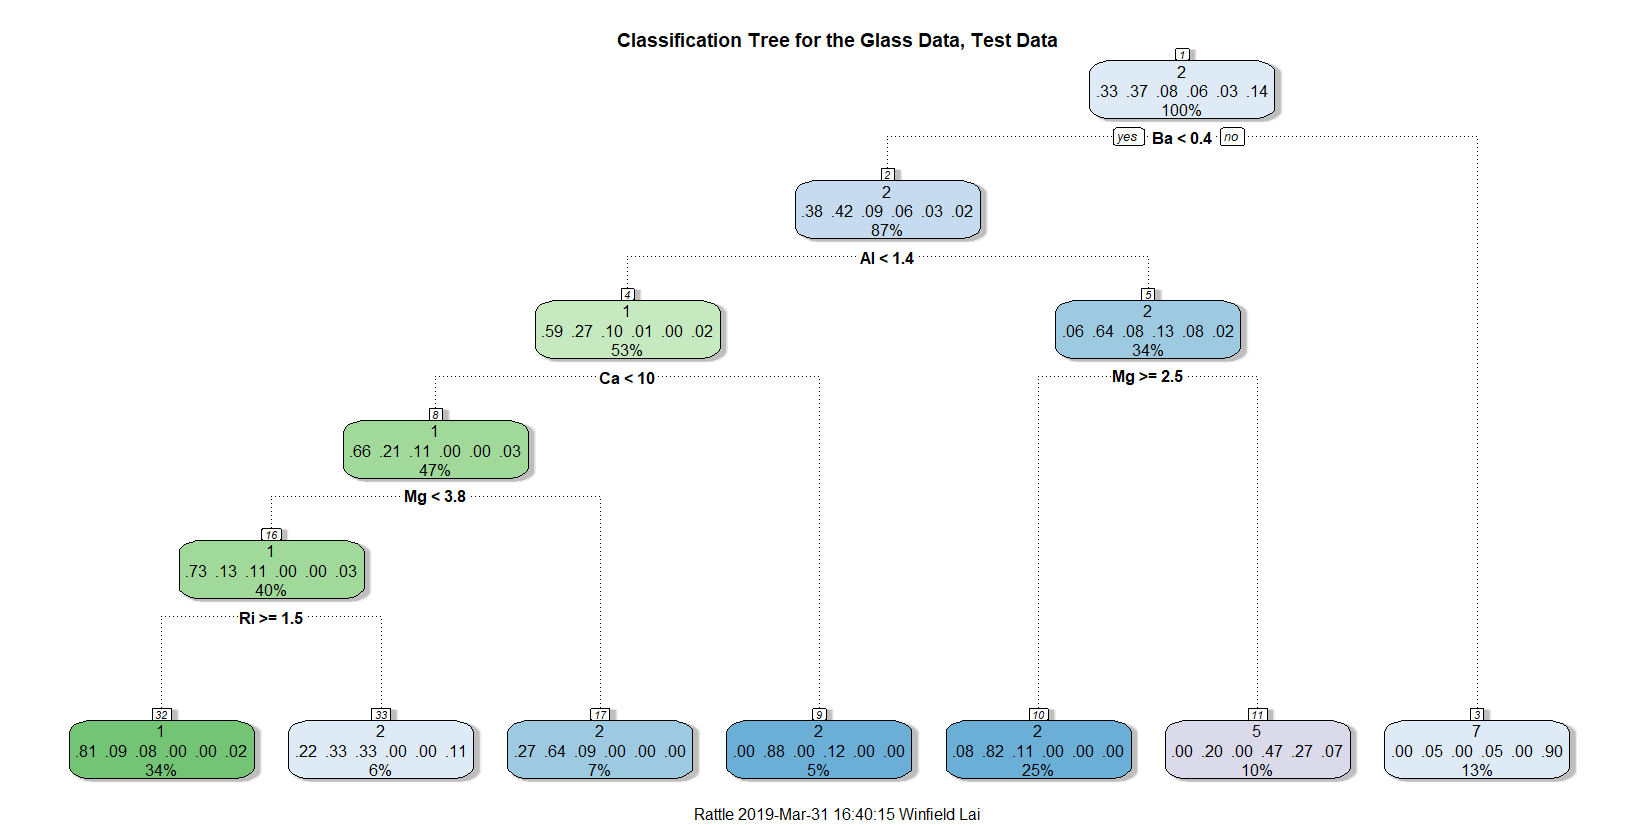
\includegraphics[width=\linewidth]{rpart_full.png}
	\caption{
		Classification tree. 4 of the nodes are relatively pure, but the other 3 are very impure. In fact, the decision tree lacks the ability to predict Type 3 and Type 6 glass. 6 out of the possible 9 attributes are used here. 
	}
	\label{f:class}
\end{figure}

		\begin{table}[ht]
		\centering
		\resizebox{!}{0.6in}{
		\begin{tabular}{rrrrr}
		  \hline
		CP & nsplit & rel error & xerror & xstd \\ 
		  \hline
		0.22 & 0.00 & 1.00 & 1.06 & 0.06 \\ 
		  0.07 & 2.00 & 0.56 & 0.58 & 0.06 \\ 
		  0.04 & 3.00 & 0.48 & 0.55 & 0.06 \\ 
		  0.01 & 5.00 & 0.40 & 0.52 & 0.06 \\ 
		  0.01 & 6.00 & 0.39 & 0.49 & 0.06 \\ 
		   \hline
		\end{tabular}}
		\resizebox{!}{0.6in}{
		\begin{tabular}{rrrrrrr}
		  \hline
		 & 1 & 2 & 3 & 5 & 6 & 7 \\ 
		  \hline
		  	1 &  12 &   4 &   1 &   0 &   1 &   0 \\ 
		  2 &   5 &  14 &   4 &   0 &   2 &   0 \\ 
		  3 &   0 &   0 &   0 &   0 &   0 &   0 \\ 
		  5 &   0 &   1 &   0 &   4 &   2 &   0 \\ 
		  6 &   0 &   0 &   0 &   0 &   0 &   0 \\ 
		  7 &   1 &   0 &   0 &   0 &   0 &   8 \\ 
		   \hline
		\end{tabular}}
		\caption{\\
		\textbf{Left:}  Classification Error table. The cross validation error (xerror) and relative error (rel error) is quite high and stays high even after considering more nodes. This is reflective of the trees poor node purity and inability to classify Type 3 and Type 6 glass.  \\
		\textbf{Right:} Confusion table for the above classification tree. As expected from Figure \ref{f:class}, we have no classifications of Type 3 or Type 6 and we have large node impurities.}
		\label{t:class}
		\end{table}


Looking at the node impurities, we see that the classification tree cannot classify Type 3 and Type 6 glass. This is reflective of the fact that types are never separated well from Type 1-2 and Type 5 respectively (Seen in Figure \ref{f:dataBasic_Vis}). We see that the KNN algorithm is able to classify all types. This is reflective of how KNN is essentially a distance measure and classification trees tries to predict the probability of labels being where they should and should not be. Overall, this indicates the classification trees are a poor choice when the data is hard to separate and KNN is a more robust choice for hard to separate data. 

According to the ARI (0.31), the classification tree is worse than both KNN methods above (0.35 and 0.98 respectively). It's interesting that the attributes chosen to split on mimic the attributes taken out for the KNN method above. The classification tree usd Ba, Al, Mg, Ca and Ri whereas the KNN method used Mg, Ak, Ba and Fe. The methods are fundamentally different since KNN uses a measure of distance for prediction and this classification trees constructed the splitters based on the Gini index, so it may not be useful to test KNN with the attributes used by the classification tree. 


\section{Conclusion}
A classification tree was outperformed by KNN for predicting classification of glass objects based on a training and test set. The removal of particular variables dramatically increased the ARI of the KNN method. If glass needs to be identified, Mg, Al, Ba and Fe should be measured in order to be analyzed by the KNN algorithm above. 

\newpage
\bibliographystyle{amsplain}
\bibliography{ref}{}




\end{document}
